\documentclass[border=4pt]{standalone}
% shared style for all PyTBA topology diagrams (\input by each standalone file)
\usepackage{mathpazo}
\usepackage{amsmath}
\usepackage{tikz}
\usetikzlibrary{positioning,arrows.meta,calc,decorations.pathreplacing,fit,backgrounds}
\tikzset{
  host/.style={draw=blue!55!black, fill=blue!7, rounded corners=2pt, align=center,
               minimum height=9mm, minimum width=22mm, font=\small},
  blk/.style={draw=black!60, fill=black!4, rounded corners=2pt, align=center,
              minimum height=8mm, font=\small},
  chan/.style={draw=orange!70!black, fill=orange!8, rounded corners=2pt, align=center,
               minimum height=9mm, font=\small},
  lossbox/.style={draw=red!70!black, fill=red!6, rounded corners=2pt, align=center, font=\footnotesize},
  data/.style={-{Stealth[length=2.2mm]}, thick},
  ack/.style={-{Stealth[length=2mm]}, dashed, black!60},
  lbl/.style={font=\footnotesize, align=center},
  brace/.style={decorate, decoration={brace, amplitude=4pt}, thick, black!70},
}

\begin{document}
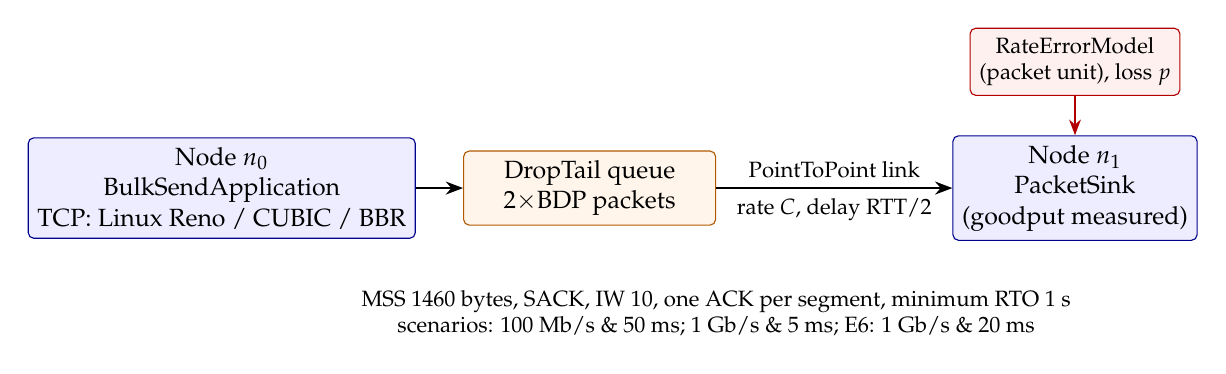
\begin{tikzpicture}
\node[host, minimum width=34mm] (n0) {Node $n_0$\\BulkSendApplication\\TCP: Linux Reno / CUBIC / BBR};
\node[chan, right=6mm of n0, minimum width=32mm] (q) {DropTail queue\\$2\times$BDP packets};
\node[host, right=30mm of q, minimum width=30mm] (n1) {Node $n_1$\\PacketSink\\(goodput measured)};
\node[lossbox, above=5mm of n1] (em) {RateErrorModel\\(packet unit), loss $p$};
\draw[data] (n0) -- (q);
\draw[data] (q) -- node[lbl, above] {PointToPoint link} node[lbl, below] {rate $C$, delay RTT/2} (n1);
\draw[-{Stealth[length=2mm]}, red!70!black] (em) -- (n1);
\node[lbl, below=7mm of q.south east, anchor=north] {MSS 1460 bytes, SACK, IW 10, one ACK per segment, minimum RTO 1 s\\
  scenarios: 100 Mb/s \& 50 ms;\ 1 Gb/s \& 5 ms;\ E6: 1 Gb/s \& 20 ms};
\end{tikzpicture}
\end{document}
